\section{Quantum Key Distribution}
\begin{itemize}
	\item Qubits used for communication are usually photons, which have a momentum \( \vec k \), and 
		an electric field \( E_x \) and \( E_y \) that propagates in the plane perpendicular to \( \vec k \). 
		The \( E_x \) vector is denoted as \( \ket*{v} \), and  \( E_y \) as \( \ket*{H} \), and this means that 
		the general electric field \( \overline E = \alpha \ket*{v} + \beta \ket*{H} \). 
	\item We can pass these photons thorugh polarizers, which only transmit light with specific oscillations.  
	\item So as a quantum circuit, it's written as:
		\begin{center}
			\begin{quantikz}
				\lstick{\( \ket*{\psi} \) } & \gate[2]{pol} & & \rstick{\( |x| \)}\\
											& & &  \rstick{\( |y| \) }
			\end{quantikz}
		\end{center}
		Only one of these channels can be measured,  
\end{itemize}
\subsection{Distributed Entanglement}
\begin{itemize}
	\item One of the ways to do quantum communication and computation
	\item It includes: 
		\begin{itemize}
			\item teleportation
			\item Secure QKD: communication
			\item Distributed quantum computation -- quantumgatsby teleportation
			\item "Blind quantum teleportation" 
		\end{itemize}
\end{itemize}
\subsubsection{QKD Secureness}
\begin{itemize}
	\item The way QKD works is a server \( \ket*{\psi} = \ket*{HV} + \ket*{VH} \), and the first qubit is sent to 
		Bob, and the second is sent to Alice: 
		\begin{center}
			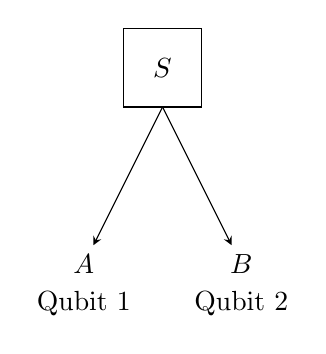
\begin{tikzpicture}
				\node (A) at (1, 0) {\(  B \)};
				\node (B) at (-1, 0) {\( A \) }; 
				\draw (-0.5, 2) rectangle node{\( S \) } (0.5, 3);
				\draw[-stealth] (0, 2) -- (A); 
				\draw[-stealth] (0, 2) -- (B);
				\draw node at (1, -0.5) {Qubit 2};
				\draw node at (-1, -0.5) {Qubit 1};
			\end{tikzpicture}
		\end{center}
	\item Classically, if an observer were to say, measure the second qubit, then send an identical copy through 
		that channel, then Alice and Bob won't be able to tell at all that the state has been measured. 

		However, if the system was quantum, this measurement is now impossible. 
	\item The proof of this is called the No cloning theorem, whose proof is below: 

		\begin{proof}
			Suppose we have an unknown state   \( \ket*{\phi} = \alpha \ket*{0} + \beta \ket*{1} \).  Now suppose 
			there is a \( U_{cl} \) (a "cloning matrix") which can clone \( \ket*{\phi} \). That is:
			\[
			\ket*{\phi}\ket*{0} \mapsto \ket*{\phi}\ket*{\phi} = \alpha^2 \ket*{00} 
			+ \beta \alpha \ket*{10} + \alpha \beta \ket*{01} + \beta^2 \ket*{11}
			\] 
			But if we do this on the initial state \( \ket*{\phi} \) : 
			\[
				(\alpha \ket*{0} + \beta \ket*{1}) \ket*{0} \mapsto \alpha \ket*{00} +\beta \ket*{11}
			\] 
			\comment{We are cloning this exactly based on what we want: we clone the information of the second 
				qubit onto the first qubit, but we see that even if we could "copy", we don't get the desired 
			product state.} 

			But this is not equal to the copied state that we should expect. Therefore, no such \( U_{cl} \) 
			can exist.
		\end{proof}
\end{itemize}
\subsection{Quantum Algorithms}
\begin{itemize}
	\item The Deutsch-Josza is a \textit{promise problem}: we are given a function \( f(x) \), and 
		it's one of two types: 
		\begin{itemize}
			\item \( f(x) \) is either constant for all \( x \) : it is either always 0 or always 1.
			\item \( f(x) \) is balanced: it is 0 half the time, \( f(x)  \) is 1 half the time. 
		\end{itemize}

		More generally, we can write \( f: \{0, 1\} ^{n} \mapsto \{0, 1\}  \), and we ask whether \( f \) is 
		constant or balanced. 
	\item For a function on \( n \) bits, this implies that the total domain space is of size \( 2^{n} \). We need to 
		measure a little more than half, or \( 2^{n} / 2 + 1 = 2^{n - 1} + 1 \) measurements in order to determine 
		the identity of \( f \).

		Quantumly, we only need a single measurement!
	\item The quantum circuit is as follows:
		\begin{center}
			\begin{quantikz}[slice all, slice titles = $\ket{\psi_\col}$ ]
				\lstick{\( \ket*{0}^{\otimes n} \)} \slice{\( \ket*{\psi_0} \) } & \gate{H^{\otimes n}} & \gate[2]{ U_f } & \gate{H^{\otimes n}} & \\
				\lstick{\( \ket*{1} \) } & \gate{H} & & & 
			\end{quantikz}
		\end{center}
		Initially, the state is in \( \ket*{\psi_0} = \ket*{0}^{\otimes n} \ket*{1} \). Then, after passing through 
		both Hadamard gates, we have: 
		\[
		\ket*{\psi_1} = \frac{1}{\sqrt{2}}\sum_x \ket*{x} \otimes \frac{1}{\sqrt{2} }(\ket*{0} - \ket*{1})
		\] 
		To explain what's happening here, here's a convenient way to denote \( H \) : 
		\[
		H = \frac{1}{\sqrt{2} }\sum_{x, y \in \{0, 1\} } (-1)^{xy}\ket*{y}\bra*{x}
		\] 
		(check for yourself that this does indeed generate the correct Hadamard matrix). Therefore, the general 
		\( n \)-qubit Hadamard gate \( H^{\otimes n} \) :
		\[
		H^{\otimes n} = \frac{1}{\sqrt{2^{n}} }\sum_{x, y \in \{0, 1\} ^{n}}(-1)^{x \cdot y}\ket*{y}\bra*{x}
		\] 
		Therefore, we can write:
		\[
			\ket*{\psi_1} = H^{\otimes n}\ket*{0^{\otimes n}} \otimes \frac{1}{\sqrt{2} }(\ket*{0} -\ket*{1})
			= \frac{1}{\sqrt{2^{n}} }\sum_x \ket*{x} \otimes \frac{1}{\sqrt{2} }(\ket*{0} - \ket*{1})
		\] 
	\item Now we send \( \ket*{\psi_1} \) through \( U_f \). What it does is it sends \( \ket*{y} \) 
		to \( \ket*{y \oplus f(x)} \). If \( y = 0 \), then we just output \( f(x) \), and if \( y = 1 \), thne 
		we output the \textit{complement} of \( f(x) \), since if \( f(x) = 1 \) then the addition modulo 2 
		would return us 0, and vice versa. Therefore, we can write \( \ket*{\psi_2} \) as: 
		\[
			\ket*{\psi_2} = \frac{1}{\sqrt{2^{n}} }\sum_x \ket*{x }\otimes \frac{1}{\sqrt{2} }
			(\ket*{f(x)} - \ket*{\overline{f(x)}})
		\] 
		If \( f(x) = 0 \), then the ancilla (the last qubit) is \( \ket*{0} - \ket*{1} \), and if \( f(x) = 1 \), 
		then the ancilla is  \( \ket*{1} - \ket*{0} = -(\ket*{0} - \ket*{1}) \). So in general, the ancilla is 
		\( (-1)^{f(x)}(\ket*{0} - \ket*{1})  \). Therefore, we can write:
		\[
		\ket*{\psi_2} = \frac{1}{\sqrt{2^{n}} } \sum_x (-1)^{f(x)}\ket*{x} \otimes \frac{1}{\sqrt{2} }(\ket*{0} - \ket*{1})
		\] 
		\comment{We can write \( (-1)^{f(x)} \) because when \( f(x) = 0 \) then \( (-1)^{f(x)} = 1 \), which doesn't
		change the product at all, but it changes when \( f(x) = 1 \), which is what we want.}
	\item Finally, we act \( H^{\otimes n} \) on the data register. Note that \( H^{\otimes n}\ket*{x} = 
		\sum_y (-1)^{xy}\ket*{y}\), so this gives us:
		\[
		\ket*{\psi_3} = \frac{1}{\sqrt{2^{n}} }\sum_y\sum_x (-1)^{f(x) + (x \cdot y)}\ket*{y} \otimes 
		\frac{1}{\sqrt{2} }(\ket*{0} - \ket*{1})
		\] 
	\item Now we measure all \( n \) qubits. If \( f(x) \) is constant, 
\end{itemize}
